% Pin the LaTeX2e kernel to a stable release. The installed lineno (v5.6/5.7,
% 2026) only patches its twocolumn support against a LaTeX2e kernel dated
% 2026-06-01 or later; on this kernel that patch still misplaces line numbers
% in review mode (acl.sty's 2012-era twocolumn hack was never designed for
% it). Rolling the kernel back to a stable pre-regression date avoids the
% conflict entirely, with no change to columns, margins, or spacing.
\RequirePackage[2024-06-01]{latexrelease}

\documentclass[11pt]{article}

% Change "review" to "final" to generate the final (sometimes called camera-ready) version.
% Change to "preprint" to generate a non-anonymous version with page numbers.
\usepackage[review]{acl}

% Standard package includes
\usepackage{times}
\usepackage{latexsym}

% For proper rendering and hyphenation of words containing Latin characters (including in bib files)
\usepackage[T1]{fontenc}

% This assumes your files are encoded as UTF8
\usepackage[utf8]{inputenc}

% This is not strictly necessary, and may be commented out,
% but it will improve the layout of the manuscript,
% and will typically save some space.
\usepackage{microtype}

% This is also not strictly necessary, and may be commented out.
% However, it will improve the aesthetics of text in
% the typewriter font.
\usepackage{inconsolata}

% Including images in your LaTeX document requires adding
% additional package(s)
\usepackage{graphicx}

% Additional packages used by this paper
\usepackage{booktabs}
\usepackage{multirow}
\usepackage{amsmath}
\usepackage{xcolor}
\usepackage{colortbl}
\usepackage{array}
\usepackage{makecell}
\usepackage{enumitem}

\DeclareMathOperator*{\argmax}{arg\,max}

\definecolor{high}{HTML}{c7e9c0}
\definecolor{mid}{HTML}{fff5c0}
\definecolor{low}{HTML}{fdd0c0}
\definecolor{best}{HTML}{74c476}

\title{Can Geography Stand In for Labeled Data in Arabic Dialect Identification?\\ A Cross-Linguistic Stress Test of Geographic $N$-Gram Interpolation}

\author{Anonymous}

\begin{document}
\maketitle

%% ──────────────────────────────────────────────────────────────────────────────
\begin{abstract}
Arabic dialect identification covers only a fraction of the Arabic speaking world, and most regions have no labeled data at all.
A natural starting point is Tobler's law, which states "\textit{everything is related to everything else, but near things are more related than distant things.}" Applying it to dialects means that nearby dialects tend to be more alike.
We test this idea directly for Arabic, then check whether it holds up by repeating the same test on six more language families.
For Arabic, we build a model for an unseen dialect from its nearest known dialects, weighted by distance.
On the NADI 2020 benchmark across 17 dialects, this recovers \textbf{63\% of oracle macro F1 with zero target labels}, the best score among all seven families we test.
For Mauritania and Somalia, two dialects missing from training entirely, our method still gives real predictions.
Repeating the protocol on German, Russian, English, Portuguese, Spanish, and French, we find that recovery is useful everywhere, from 26\% to 63\%.
But the correlation between geography and similarity does not predict which families benefit: neither its size (Spearman $\rho{=}{-}0.21$) nor its sign ($\rho{=}{-}0.71$, $p{=}0.07$) gives a rule a practitioner could trust.
The lesson for Arabic dialect identification is good news with a catch.
The code available at: \url{https://anonymous.4open.science/r/counterplay-A37E}
\end{abstract}

%% ──────────────────────────────────────────────────────────────────────────────
\section{Introduction}
\label{sec:intro}

Arabic dialect identification (DID) assigns informal text to one of the many regional varieties spoken across the Arab world.
The task matters for machine translation, sentiment analysis, and information retrieval, where treating Arabic as a single language hides large differences between, say, Peninsular and Maghrebi usage \cite{zaidan-callison-burch-2014-arabic}.
Resources such as the MADAR corpus \cite{bouamor-etal-2018-madar} and dialect identification datasets like DSL-TL \cite{haapanen-etal-2023-dsltl} have pushed coverage forward, yet systems exist for only a fraction of Arabic's dialect continuum: the largest shared benchmark, NADI, covers under 20 of more than 20 dialect-bearing countries, and most regions have no labeled data at all.

The core problem is annotation cost.
Building a DID system for a new dialect requires collecting and labeling text from that region, which may be slow, expensive, or impossible for an under-resourced variety, a challenge that mirrors the broader difficulty of language identification for low-resource varieties on noisy web text \cite{caswell-etal-2020-language}.
\textbf{Geographic proximity} is a natural guide: if nearby dialects are more similar, a model trained on neighboring regions can stand in for an unseen one.
This idea, grounded in Tobler's first law of geography \cite{nerbonne-heeringa-1997-measuring}, has direct support for Arabic: \citet{alsudais-etal-2022-similarities} found that geographically closer Arabic dialects have more similar $n$-gram profiles.
What is missing is a working system built on that finding, evaluated against a real benchmark, and a sense of how much to trust it.

We supply both.
First, we build and evaluate a geographic interpolation system for Arabic dialect identification on the NADI 2020 benchmark, including a true zero shot test on dialects entirely absent from training and an annotation cost analysis that tells practitioners how many labels it takes to beat the zero shot baseline.
Second, because a result from one language family could be an accident of Arabic's particular history rather than a general property of geographic interpolation, we stress-test the method on six more families that spread across the globe in different ways: through \textbf{in situ evolution} (communities stay in place and dialects drift through contact with neighbors, as in Arabic itself), \textbf{colonial spread} (Spanish, Portuguese, and English carried to the Americas from a recent common European source), \textbf{imperial spread} (Russian carried across Central Asia by Soviet rule, native in Russia but imposed elsewhere), and \textbf{mixed} settlement (French, spanning in situ European varieties and colonial African ones).
If the geographic--linguistic correlation $r$ that \citet{alsudais-etal-2022-similarities} measured for Arabic could be computed on unlabeled data and used to decide, ahead of time, whether geographic interpolation is worth deploying for a new dialect, that would turn their finding into a general recipe.
We test whether it does.
We find that it does not: $r$ is not a reliable advance signal even though the method itself works well for Arabic.

Our mixture model builds a character $n$-gram model for an unseen country from its $k$ nearest known countries, weighted by inverse geographic distance between country centroids (Section~\ref{sec:method}).

Our contributions are:
\begin{enumerate}[leftmargin=*,topsep=2pt]
\item The first system-level evaluation of geographic interpolation for Arabic DID against a real external benchmark (NADI 2020, 17 dialects): 63\% of oracle macro F1 recovered with zero target labels, the strongest result of any family we test.
\item A true zero shot evaluation on Mauritanian and Somali Arabic, dialects absent from all training data, where our method is the only one to give non-degenerate predictions, plus an annotation cost analysis showing that around 10 labeled tweets per dialect beat the zero shot baseline.
\item A six-family stress test (German, Russian, English, Portuguese, Spanish, French; 58 further varieties) of whether the Arabic result generalizes as a recipe. Recovery is a usable proxy everywhere (26--63\%), but the geographic--linguistic correlation $r$ does \emph{not} predict which families benefit: neither $|r|$ (Spearman $\rho{=}{-}0.21$) nor signed $r$ ($\rho{=}{-}0.71$, $p{=}0.07$) gives a reliable advance rule. Arabic's success cannot be safely assumed to transfer to the next untested language.
\end{enumerate}

%% ──────────────────────────────────────────────────────────────────────────────
\section{Related Work}
\label{sec:related}

\paragraph{Dialect and language identification.}
Character $n$-gram models have been strong baselines for variety discrimination since \citet{cavnar-trenkle-1994-ngram} and remain competitive \cite{tiedemann-ljubesic-2012-efficient,zampieri-etal-2014-report}.
For Arabic, \citet{salameh-etal-2018-fine} use smoothed $n$-gram language models for fine grained DID.
The NADI series \cite{abdul-mageed-etal-2020-nadi, abdul-mageed-etal-2024-nadi} tests country level Arabic DID including an unseen dialect track.
See \citet{jauhiainen-etal-2019-automatic} for a full survey.

\paragraph{Geography and dialect variation.}
Dialectometry \cite{nerbonne-heeringa-1997-measuring,nerbonne-2010-dialectometry} measures how dialects vary across space.
\citet{eisenstein-etal-2010-latent} showed that Twitter location correlates with word choice, and \citet{lui-cook-2013-classifying} used geotagged $n$-gram models for English national varieties.
For Arabic, \citet{alsudais-etal-2022-similarities} found a negative correlation between Haversine distance and dialect similarity and called for using this to transfer models.
We test that idea and probe its limits across six more families.

\paragraph{Zero shot cross-dialect transfer.}
Zero shot cross lingual transfer is well studied for transformers \cite{inoue-etal-2021-interplay}, but geographic structure has not been used as a guide.
NADI 2024 \cite{abdul-mageed-etal-2024-nadi} added an unseen dialect track, where participants used transformer fine tuning and prompting.
This work instead maps when geographic proximity is, and is not, a reliable guide for building dialect models.

\paragraph{Weak geographic supervision.}
CC-TLD filtering has been used as a noisy geographic label for web text \cite{nllb-team-2022-language}.
Geotagged social media has been used to study lexical diffusion \cite{eisenstein-etal-2010-latent} and national variety differences \cite{lui-cook-2013-classifying}.
We bring both sources together under a unified evaluation framework, using CC-TLD web text as a similar, if noisier, geographic label for the six families beyond Arabic.

%% ──────────────────────────────────────────────────────────────────────────────
\section{Data}
\label{sec:data}

\subsection{Arabic: Geotagged Twitter}

We use geotagged tweets from \citet{abdelrahman-rezk-2021}: 18 countries, 440{,}000 tweets, users assigned by their declared Twitter location.
Twitter captures \emph{colloquial} Arabic because of diglossia.
Arabic has two coexisting registers: Modern Standard Arabic (MSA), used in formal writing and broadcast media, and a set of regional spoken dialects that differ enough to impede mutual comprehension across regions.
Because social media is informal, speakers write in their own dialect.
Peninsular Arabic, Levantine Arabic, and Maghrebi Arabic are phonologically and lexically distinct in these colloquial texts, making geotagged Twitter a reliable source of dialectal signal.

\subsection{CC-TLD Web Text}

For all other six languages, we use country-code top-level domain (CC-TLD) filtered documents from the mc4 multilingual web corpus \cite{nllb-team-2022-language}.
Each document is assigned to a country based on its URL domain: a document from a \texttt{.de} domain is assigned to Germany, one from \texttt{.mx} to Mexico, and so on.
We collect up to 10{,}000 documents per country, cut each to 500 characters for efficiency, and remove any country with fewer than 80 documents.

CC-TLD is a noisy signal: a \texttt{.de} domain does not guarantee native German content, and diaspora communities produce off-country text.
Despite this noise, the aggregate signal across thousands of documents is strong enough to produce distinct character $n$-gram profiles per country.
Unlike geotagged Twitter, mc4 web text leans toward \emph{formal written} language, which turns out to matter for whether geographic structure is present.
We return to this in Section~\ref{sec:register}.

\subsection{Dataset Overview}

Table~\ref{tab:data} summarizes the data for all seven language families.
Arabic varieties are trained on the full available data.
CC-TLD varieties are capped at 10{,}000 documents each.
Country centroids are computed as population-weighted geographic midpoints, taken from public geographic databases.

\begin{table}[t]
\centering
\small
\setlength{\tabcolsep}{4pt}
\begin{tabular}{llrrc}
\toprule
\textbf{Language} & \textbf{Source} & \textbf{\#var} & \textbf{Docs} & \textbf{Register} \\
\midrule
Arabic     & Twitter    & 17 & 440K & colloquial \\
English    & mc4 CC-TLD & 11 &  95K & formal \\
French     & mc4 CC-TLD & 13 &  85K & formal \\
Spanish    & mc4 CC-TLD & 17 &  51K & formal \\
Portuguese & mc4 CC-TLD &  3 &  65K & formal \\
Russian    & mc4 CC-TLD &  9 &  75K & formal \\
German     & mc4 CC-TLD &  5 &  38K & formal \\
\bottomrule
\end{tabular}
\caption{Dataset overview. \#var = varieties scored in the leave one out macro (oracle F1 ${>}0.01$).
  Arabic trains 18 and Spanish trains 19, but Bahrain, Panama, and Paraguay have near-zero oracle and are dropped.
  Docs = total documents used (capped at 10{,}000 per variety for CC-TLD languages).
  Arabic uses geotagged Twitter.
  All other languages use CC-TLD filtered web text from mc4.}
\label{tab:data}
\end{table}

%% ──────────────────────────────────────────────────────────────────────────────
\section{Method}
\label{sec:method}

\subsection{Character $n$-Gram Language Models}

We model each geographic variety as a character $n$-gram language model with interpolated Kneser-Ney smoothing \cite{chen-goodman-1999-empirical}, order $n{=}4$.
Character $n$-grams capture subword patterns that differ across dialects: spelling conventions, affixes, clitics, and script-specific ligatures.
They are script agnostic and require no tokenizer, making them easy to deploy across the seven languages in this study.
One model is trained per variety from that variety's documents.

At test time, text $t$ is assigned to the variety with the highest log-linear score:
\begin{equation}
  \hat{c} \;=\; \argmax_{c} \; \bigl[\log P(t \mid c) + \log P(c)\bigr],
  \label{eq:classifier}
\end{equation}
where $P(c)$ is a prior over varieties estimated from training document counts.

\subsection{Geographic Interpolation and Correlation}
\label{sec:corr_def}

For an unseen country $c^*$, we build a synthesized model as a weighted mixture over the $k{=}5$ nearest known countries:
%
\begin{equation}
  \hat{P}(w \mid c^*) \;=\; \sum_{i \in \mathcal{N}_k(c^*)}
    \alpha_i \, P(w \mid c_i),
  \label{eq:mixture}
\end{equation}
%
with $\alpha_i \propto 1/d(c^*, c_i)$, where $d(\cdot,\cdot)$ is the Haversine distance between country centroids.
The interpolated cell takes the average log prior of its source countries.
This requires no labeled data from $c^*$, only its location.

Whether this works depends on whether geographic distance correlates with linguistic similarity.
We measure this via the Pearson correlation $r$ over all $\binom{V}{2}$ country pairs in a family.
For each pair $(c_i, c_j)$ we compute the Haversine distance $d_{ij}$ and the cosine similarity $s_{ij}$ between $n$-gram probability vectors:
\begin{equation}
  s_{ij} = \frac{\mathbf{p}_i \cdot \mathbf{p}_j}
                {\|\mathbf{p}_i\|\,\|\mathbf{p}_j\|},\quad
  r \;=\; \mathrm{Pearson}\!\bigl(\{d_{ij}\},\, \{s_{ij}\}\bigr),
  \label{eq:corr}
\end{equation}
where $\mathbf{p}_c$ is the vector of $n$-gram log probabilities under model $c$.
Negative $r$ means closer varieties are more similar (Tobler's dialectal law holds).
Positive $r$ means more distant varieties are more alike.
Near-zero $r$ means distance carries no information about similarity.

\subsection{Evaluation Protocol}

\paragraph{Leave one out (LOO).}
For Arabic, we hold out each of 18 countries in turn and test the full 18-class classifier on the NADI 2020 development set (4{,}957 tweets, external benchmark).
For all other languages, we use intrinsic LOO: each country's documents are split 80\% train / 20\% test, and we test the held out country against a classifier trained on the rest.

We report macro F1 in two conditions.
The \emph{oracle} classifier is trained with the held out country's own data (the upper bound).
The \emph{geo} classifier replaces the held out country with the geographic mixture from Eq.~\ref{eq:mixture} (the zero shot system).
\textbf{Recovery} = geo macro F1 / oracle macro F1 measures how much of the oracle performance the zero shot system achieves.

\paragraph{True zero shot.}
For Mauritania and Somalia, present in NADI 2020 but absent from our Arabic training data, we add a built cell to the 18-cell system and test directly.

\paragraph{Annotation cost.}
We train supervised $n$-gram models on $N$ labeled Arabic tweets per variety (varying $N$) and compare against the zero shot baseline to find the crossover point.

%% ──────────────────────────────────────────────────────────────────────────────
\section{Results}
\label{sec:results}

\subsection{Cross-Language Summary}
\label{sec:summary}

Table~\ref{tab:summary} shows the LOO results for all seven language families alongside the geographic--linguistic correlation $r$.

\begin{table}[t]
\centering
\footnotesize
\setlength{\tabcolsep}{3pt}
\begin{tabular}{l p{2.1cm} r r r r}
\toprule
\textbf{Lang.} & \textbf{Type} & $r$ &
  \textbf{\#v} & \textbf{Oracle} & \textbf{Rec.} \\
\midrule
Arabic    & in situ colloquial  & $-$0.43 & 17 & 0.193 & \textbf{63\%} \\
German    & in situ written     & $+$0.30 &  5 & 0.704 & \textbf{57\%} \\
English   & colonial spread     & $+$0.03 & 11 & 0.532 & \textbf{48\%} \\
Russian   & imperial spread     & $+$0.33 &  9 & 0.755 & \textbf{45\%} \\
French    & mixed EU+Africa     & $-$0.14 & 13 & 0.758 & \textbf{45\%} \\
Portug.   & colonial (few)      & $+$0.50 &  3 & 0.699 & \textbf{33\%} \\
Spanish   & colonial (many)     & $+$0.37 & 17 & 0.368 & \textbf{26\%} \\
\bottomrule
\end{tabular}
\caption{Cross-language LOO summary.
  $r$ = Pearson correlation of pairwise cosine similarity vs.\ Haversine distance (Eq.~\ref{eq:corr}).
  Negative $r$ means closer varieties are more similar.
  Rec.\ = geo macro F1 / oracle macro F1.
  Sorted by recovery.}
\label{tab:summary}
\end{table}

Two things stand out.
\emph{First}, the method is a usable proxy everywhere.
Recovery ranges from 26\% to 63\% of oracle with no target labels, and no family fails outright.
\emph{Second}, $r$ does not order the families.
Arabic ($r{=}{-}0.43$) and Portuguese ($r{=}{+}0.50$) have the two largest $|r|$ values, yet sit at opposite ends of the recovery range (63\% and 33\%).
English ($r{=}{+}0.03$, almost no correlation) recovers 48\%, more than Russian and Spanish, which have much larger $|r|$.
The one weak trend is by sign, not magnitude: the two families with $r{<}0$ (Arabic, French) land above the positive ones on average.
Section~\ref{sec:abs_r} shows that neither reading holds up statistically.

\subsection{Correlation Plots}
\label{sec:corr}

Figure~\ref{fig:corr} plots pairwise cosine similarity of $n$-gram profiles against Haversine distance for all seven language families.

\begin{figure*}[t]
\centering
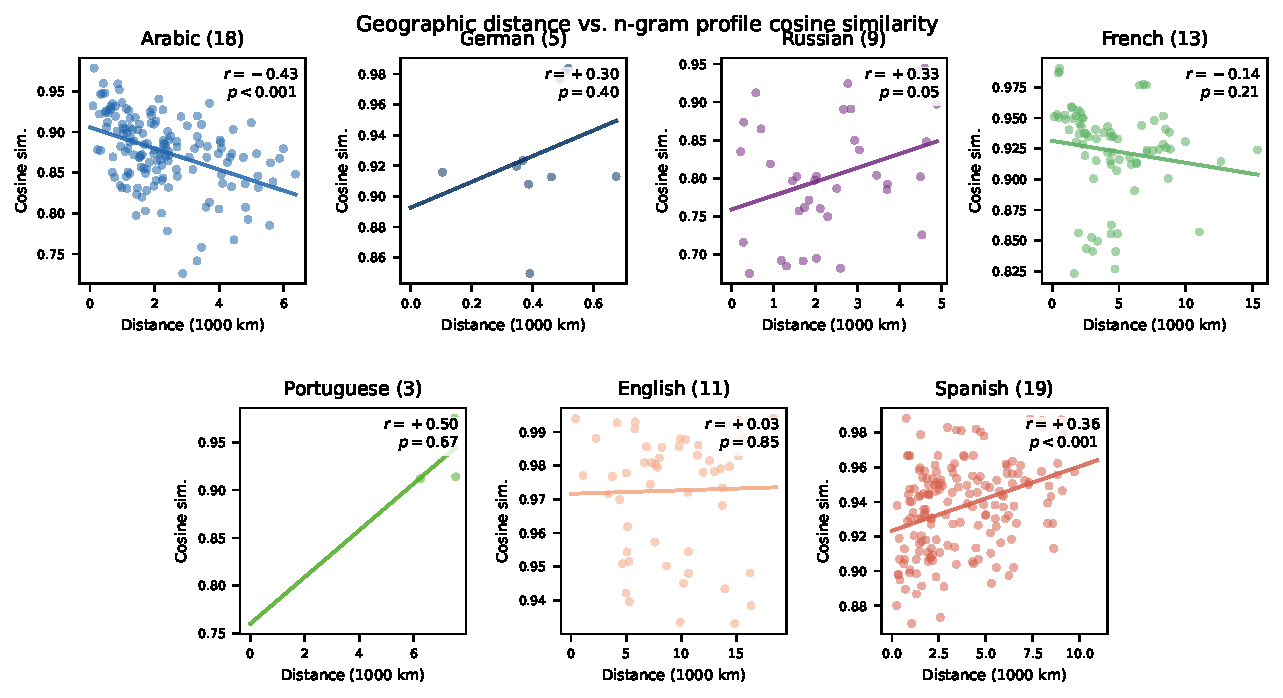
\includegraphics[width=\textwidth]{figures/corr_plot.pdf}
\caption{Geographic distance vs.\ $n$-gram profile cosine similarity across seven language families.
  Arabic ($r{=}{-}0.43$) and French ($r{=}{-}0.14$) show $r{<}0$ (closer varieties more similar).
  The rest show $r{>}0$ or $r{\approx}0$.
  Panel counts include all varieties with enough training data.}
\label{fig:corr}
\end{figure*}

Arabic's negative correlation ($r{=}{-}0.43$, $p{<}0.001$) confirms \citet{alsudais-etal-2022-similarities}: nearby Arabic varieties are genuinely more alike.
The geotagged Twitter data captures colloquial speech, where dialectal signal is strong.

German's correlation is positive but modest ($r{=}{+}0.30$).
Germany, Austria, and Switzerland are all in situ Germanic varieties that have changed together over centuries.
The data source matters here: mc4 web text tends toward \emph{Standard German} regardless of country, which flattens the regional features that distinguish Bavarian, Alemannic, and Swiss German in spoken language.

French ($r{=}{-}0.14$, $p{>}0.05$) and English ($r{=}{+}0.03$) show almost no relationship.
The French family covers European varieties (FR, BE, CH, LU), North African ones (MA, DZ, TN), West African ones (SN, CI, CM, CD), and Canadian.
Distance tells us little here, because a European and African pair at 5{,}000\,km can be more alike than two African pairs at 1{,}000\,km.
Yet, as the next sections show, both families still recover 45--48\% of oracle.
Weak correlation does not mean the proxy is useless.

\subsection{Arabic: In Situ with Colloquial Data}
\label{sec:arabic}

Table~\ref{tab:loo} shows per country Arabic LOO.
Geographic interpolation reaches macro F1 of \textbf{0.121} against an oracle of \textbf{0.193} (63\% recovery).

\begin{table}[t]
\centering
\small
\setlength{\tabcolsep}{4.5pt}
\begin{tabular}{lrrrr}
\toprule
\textbf{Country} & \textbf{Oracle} & \textbf{Geo-5} & \textbf{Dist.} & \textbf{Rec.} \\
\midrule
\rowcolor{best}
UAE (AE)          & 0.097 & 0.125 &  323\,km & 129\% \\
\rowcolor{best}
Saudi Arabia (SA) & 0.210 & 0.259 &  602\,km & 123\% \\
\rowcolor{best}
Syria (SY)        & 0.095 & 0.111 &  293\,km & 117\% \\
\rowcolor{best}
Iraq (IQ)         & 0.232 & 0.227 &  511\,km &  98\% \\
\rowcolor{high}
Morocco (MA)      & 0.123 & 0.113 &  947\,km &  92\% \\
\rowcolor{high}
Algeria (DZ)      & 0.267 & 0.225 &  947\,km &  84\% \\
\rowcolor{high}
Tunisia (TN)      & 0.140 & 0.105 &  991\,km &  75\% \\
\rowcolor{high}
Yemen (YE)        & 0.153 & 0.115 &  989\,km &  75\% \\
\rowcolor{high}
Palestine (PS)    & 0.098 & 0.059 &  126\,km &  60\% \\
\rowcolor{mid}
Oman (OM)         & 0.189 & 0.108 &  379\,km &  57\% \\
\rowcolor{mid}
Qatar (QA)        & 0.073 & 0.040 &   90\,km &  55\% \\
\rowcolor{mid}
Kuwait (KW)       & 0.074 & 0.040 &  465\,km &  54\% \\
\rowcolor{mid}
Egypt (EG)        & 0.567 & 0.291 &  689\,km &  51\% \\
\rowcolor{mid}
Jordan (JO)       & 0.111 & 0.047 &  126\,km &  42\% \\
\rowcolor{mid}
Libya (LY)        & 0.297 & 0.107 & 1123\,km &  36\% \\
\rowcolor{low}
Lebanon (LB)      & 0.234 & 0.058 &  232\,km &  25\% \\
\rowcolor{low}
Sudan (SD)        & 0.319 & 0.020 & 1258\,km &   6\% \\
\midrule
Bahrain (BH)      & 0.000 & 0.000 &   90\,km & --- \\
\midrule
\textbf{Macro}$^\dagger$
  & \textbf{0.193} & \textbf{0.121} & --- & \textbf{63\%} \\
\bottomrule
\end{tabular}
\caption{Arabic LOO on NADI 2020 dev (4{,}957 tweets, 18 countries).
  Dist.\ = Haversine to nearest training country.
  Rec.\ = Geo-5 / Oracle.
  $\dagger$~Macro excludes Bahrain (oracle $\approx$ 0).
  Shading: \colorbox{best}{$\geq$95\%}, \colorbox{high}{60--94\%}, \colorbox{mid}{35--59\%}, \colorbox{low}{$<$35\%}.}
\label{tab:loo}
\end{table}

Recovery varies widely and tracks geographic embeddedness.
The Peninsular and Levant cluster recovers best.
UAE (129\%), Saudi Arabia (123\%), and Syria (117\%) even beat their own oracle, because their Twitter training data is noisier than their neighbors' and the mixture borrows cleaner signal.
Saudi Arabia and Iraq (98\%) are surrounded by near-identical varieties.
Lebanon (25\%) is a clear exception.
It sits only 232\,km from Palestine yet recovers poorly.
Centuries of Phoenician, Aramaic, and French contact have pulled Lebanese Arabic away from its geographic position.
Sudan (6\%) is the most isolated case.
Its nearest model country (Egypt, 1{,}258\,km) competes rather than helps.
This within-Arabic spread, from 6\% to over 100\%, is wider than the spread \emph{across} whole families, a first sign that geographic distance alone is a coarse guide.

\subsection{Other Language Families}
\label{sec:multi}

Tables~\ref{tab:de}--\ref{tab:es} show per country LOO for German, Russian, English, French, Portuguese, and Spanish.

\begin{table}[t]
\centering
\small
\setlength{\tabcolsep}{4.5pt}
\begin{tabular}{lrrrr}
\toprule
\textbf{CC} & \textbf{Oracle} & \textbf{Geo} & \textbf{Dist.} & \textbf{Rec.}\\
\midrule
\rowcolor{mid}  AT & 0.711 & 0.375 &  387\,km & 53\% \\
\rowcolor{high} CH & 0.659 & 0.412 &  104\,km & 63\% \\
\rowcolor{high} DE & 0.610 & 0.414 &  462\,km & 68\% \\
\rowcolor{mid}  LI & 0.737 & 0.427 &  104\,km & 58\% \\
\rowcolor{mid}  LU & 0.805 & 0.364 &  368\,km & 45\% \\
\midrule
\textbf{Macro} & \textbf{0.704} & \textbf{0.399} & --- & \textbf{57\%}\\
\bottomrule
\end{tabular}
\caption{German per country LOO (CC-TLD intrinsic evaluation).
  Dist.\ = Haversine to nearest training country.
  Shading: \colorbox{best}{$\geq$95\%}, \colorbox{high}{60--94\%}, \colorbox{mid}{35--59\%}, \colorbox{low}{$<$35\%}.}
\label{tab:de}
\end{table}

\begin{table}[t]
\centering
\small
\setlength{\tabcolsep}{4.5pt}
\begin{tabular}{lrrrr}
\toprule
\textbf{CC} & \textbf{Oracle} & \textbf{Geo} & \textbf{Dist.} & \textbf{Rec.}\\
\midrule
\rowcolor{mid}  AM & 0.752 & 0.355 &  221\,km & 47\% \\
\rowcolor{mid}  AZ & 0.824 & 0.408 &  221\,km & 49\% \\
\rowcolor{low}  BY & 0.728 & 0.242 &  579\,km & 33\% \\
\rowcolor{mid}  GE & 0.742 & 0.398 &  279\,km & 54\% \\
\rowcolor{mid}  KG & 0.838 & 0.396 &  927\,km & 47\% \\
\rowcolor{mid}  KZ & 0.759 & 0.282 &  927\,km & 37\% \\
\rowcolor{mid}  MD & 0.863 & 0.354 &  291\,km & 41\% \\
\rowcolor{high} RU & 0.561 & 0.345 & 3041\,km & 61\% \\
\rowcolor{mid}  UA & 0.725 & 0.303 &  291\,km & 42\% \\
\midrule
\textbf{Macro} & \textbf{0.755} & \textbf{0.343} & --- & \textbf{45\%}\\
\bottomrule
\end{tabular}
\caption{Russian per country LOO (CC-TLD intrinsic evaluation).
  Dist.\ = Haversine to nearest training country.
  Shading: \colorbox{best}{$\geq$95\%}, \colorbox{high}{60--94\%}, \colorbox{mid}{35--59\%}, \colorbox{low}{$<$35\%}.}
\label{tab:ru}
\end{table}

\begin{table}[t]
\centering
\small
\setlength{\tabcolsep}{4.5pt}
\begin{tabular}{lrrrr}
\toprule
\textbf{CC} & \textbf{Oracle} & \textbf{Geo} & \textbf{Dist.} & \textbf{Rec.}\\
\midrule
\rowcolor{mid}  AU & 0.416 & 0.180 & 4155\,km & 43\% \\
\rowcolor{mid}  CA & 0.480 & 0.236 & 2257\,km & 49\% \\
\rowcolor{high} GB & 0.404 & 0.261 &  403\,km & 65\% \\
\rowcolor{mid}  GH & 0.633 & 0.339 & 1075\,km & 54\% \\
\rowcolor{mid}  IE & 0.522 & 0.270 &  403\,km & 52\% \\
\rowcolor{mid}  IN & 0.593 & 0.213 & 5010\,km & 36\% \\
\rowcolor{mid}  KE & 0.619 & 0.324 & 3388\,km & 52\% \\
\rowcolor{high} NG & 0.650 & 0.394 & 1075\,km & 61\% \\
\rowcolor{mid}  NZ & 0.498 & 0.227 & 4155\,km & 46\% \\
\rowcolor{mid}  US & 0.568 & 0.245 & 2257\,km & 43\% \\
\rowcolor{low}  ZA & 0.465 & 0.145 & 3753\,km & 31\% \\
\midrule
\textbf{Macro} & \textbf{0.532} & \textbf{0.258} & --- & \textbf{48\%}\\
\bottomrule
\end{tabular}
\caption{English per country LOO (CC-TLD intrinsic evaluation).
  Dist.\ = Haversine to nearest training country.
  Shading: \colorbox{best}{$\geq$95\%}, \colorbox{high}{60--94\%}, \colorbox{mid}{35--59\%}, \colorbox{low}{$<$35\%}.}
\label{tab:en}
\end{table}

\begin{table}[t]
\centering
\small
\setlength{\tabcolsep}{4.5pt}
\begin{tabular}{lrrrr}
\toprule
\textbf{CC} & \textbf{Oracle} & \textbf{Geo} & \textbf{Dist.} & \textbf{Rec.}\\
\midrule
\rowcolor{mid}  BE & 0.574 & 0.273 &  159\,km & 48\% \\
\rowcolor{mid}  CA & 0.764 & 0.300 & 8784\,km & 39\% \\
\rowcolor{mid}  CD & 0.916 & 0.369 & 1642\,km & 40\% \\
\rowcolor{mid}  CH & 0.668 & 0.303 &  368\,km & 45\% \\
\rowcolor{mid}  CI & 0.781 & 0.410 & 1253\,km & 52\% \\
\rowcolor{mid}  CM & 0.776 & 0.409 & 1642\,km & 53\% \\
\rowcolor{mid}  DZ & 0.842 & 0.328 &  947\,km & 39\% \\
\rowcolor{high} FR & 0.513 & 0.325 &  539\,km & 63\% \\
\rowcolor{mid}  LU & 0.773 & 0.307 &  159\,km & 40\% \\
\rowcolor{mid}  MA & 0.745 & 0.360 &  947\,km & 48\% \\
\rowcolor{mid}  MG & 0.856 & 0.331 & 3088\,km & 39\% \\
\rowcolor{mid}  SN & 0.847 & 0.409 & 1253\,km & 48\% \\
\rowcolor{mid}  TN & 0.797 & 0.308 &  991\,km & 39\% \\
\midrule
\textbf{Macro} & \textbf{0.758} & \textbf{0.341} & --- & \textbf{45\%}\\
\bottomrule
\end{tabular}
\caption{French per country LOO (CC-TLD intrinsic evaluation).
  Dist.\ = Haversine to nearest training country.
  Shading: \colorbox{best}{$\geq$95\%}, \colorbox{high}{60--94\%}, \colorbox{mid}{35--59\%}, \colorbox{low}{$<$35\%}.}
\label{tab:fr}
\end{table}

\begin{table}[t]
\centering
\small
\setlength{\tabcolsep}{4.5pt}
\begin{tabular}{lrrrr}
\toprule
\textbf{CC} & \textbf{Oracle} & \textbf{Geo} & \textbf{Dist.} & \textbf{Rec.}\\
\midrule
\rowcolor{high} AO & 0.381 & 0.256 & 6251\,km & 67\% \\
\rowcolor{low}  BR & 0.874 & 0.228 & 7511\,km & 26\% \\
\rowcolor{low}  PT & 0.843 & 0.218 & 6251\,km & 26\% \\
\midrule
\textbf{Macro} & \textbf{0.699} & \textbf{0.234} & --- & \textbf{33\%}\\
\bottomrule
\end{tabular}
\caption{Portuguese per country LOO (CC-TLD intrinsic evaluation).
  Dist.\ = Haversine to nearest training country.
  Shading: \colorbox{best}{$\geq$95\%}, \colorbox{high}{60--94\%}, \colorbox{mid}{35--59\%}, \colorbox{low}{$<$35\%}.}
\label{tab:pt}
\end{table}

\begin{table}[t]
\centering
\small
\setlength{\tabcolsep}{4.5pt}
\begin{tabular}{lrrrr}
\toprule
\textbf{CC} & \textbf{Oracle} & \textbf{Geo} & \textbf{Dist.} & \textbf{Rec.}\\
\midrule
\rowcolor{mid} AR & 0.459 & 0.249 &  762\,km & 54\% \\
\rowcolor{mid} BO & 0.208 & 0.094 &  958\,km & 45\% \\
\rowcolor{mid} CL & 0.580 & 0.208 &  762\,km & 36\% \\
\rowcolor{low} CO & 0.529 & 0.082 &  833\,km & 16\% \\
\rowcolor{low} CR & 0.154 & 0.034 &  355\,km & 22\% \\
\rowcolor{low} CU & 0.488 & 0.050 &  959\,km & 10\% \\
\rowcolor{low} DO & 0.422 & 0.109 &  959\,km & 26\% \\
\rowcolor{low} EC & 0.400 & 0.131 &  833\,km & 33\% \\
\rowcolor{mid} ES & 0.399 & 0.142 & 6728\,km & 36\% \\
\rowcolor{low} GT & 0.054 & 0.000 &  263\,km &  0\% \\
\rowcolor{low} HN & 0.263 & 0.000 &  278\,km &  0\% \\
\rowcolor{low} MX & 0.492 & 0.050 & 1560\,km & 10\% \\
\rowcolor{mid} NI & 0.245 & 0.086 &  278\,km & 35\% \\
\rowcolor{low} PE & 0.548 & 0.089 &  896\,km & 16\% \\
\rowcolor{low} SV & 0.182 & 0.000 &  263\,km &  0\% \\
\rowcolor{mid} UY & 0.392 & 0.143 & 1043\,km & 36\% \\
\rowcolor{mid} VE & 0.443 & 0.155 &  875\,km & 35\% \\
\midrule
\textbf{Macro} & \textbf{0.368} & \textbf{0.095} & --- & \textbf{26\%}\\
\bottomrule
\end{tabular}
\caption{Spanish per country LOO (CC-TLD intrinsic evaluation).
  Dist.\ = Haversine to nearest training country.
  Macro excludes countries with oracle ${\leq}0.01$ (Panama, Paraguay).
  Shading: \colorbox{best}{$\geq$95\%}, \colorbox{high}{60--94\%}, \colorbox{mid}{35--59\%}, \colorbox{low}{$<$35\%}.}
\label{tab:es}
\end{table}

\paragraph{German (57\%).}
The best non-Arabic recovery, 45--68\% across five compact Central European varieties.
Germany itself reaches 68\%.
The variety set is coherent: mc4 documents from Germany, Austria, and Switzerland all lean toward written Standard German, so any neighbor is a decent stand-in.

\paragraph{Russian (45\%).}
Former Soviet varieties recover at a moderate, even level (33--61\%).
Russia itself reaches 61\% and Georgia 54\%, with no obvious advantage for the geographically tight Caucasus cluster (Armenia, Azerbaijan around 48\%) over the distant ones.
Distance does not order the outcomes.

\paragraph{English (48\%).}
Eleven colonial varieties recover evenly (31--65\%).
Britain (65\%) and Nigeria (61\%) recover best, South Africa (31\%) least.
There is no clean split between the Anglosphere core and the African or Asian varieties, which the near-zero correlation ($r{=}{+}0.03$) already foreshadows.

\paragraph{French (45\%).}
Despite the most diverse variety set, French recovers as well as English (39--63\%).
European French (FR 63\%) tops the list and the African varieties (CI 52\%, CM 53\%, SN 48\%) are not far behind.
The earlier intuition that mixing European and African French should fail does not hold once the classifier is scored correctly.

\paragraph{Portuguese (33\%).}
Only three varieties, and the worst recovery of the six, which is the sharpest counterexample to the $|r|$ story: Portuguese has the largest $|r|$ of all (0.50) yet the second lowest recovery.
Angola recovers 67\% but Brazil and Portugal only 26\% each, because Brazil dominates any mixture it joins and is itself distinct from the European standard.

\paragraph{Spanish (26\%).}
Seventeen colonial varieties, the lowest macro recovery.
Outcomes range from 0\% (three small Central American varieties the mixture never predicts) to 54\% (Argentina), with no link to distance.

\subsection{True Zero Shot: Varieties Absent from Training}

Mauritania and Somalia appear in NADI 2020 but are absent from our Arabic training data.
Adding synthesized cells, Mauritania reaches a geo F1 of 0.018 (40 test items, 1{,}334\,km from Morocco) and Somalia 0.025 (51 items, 1{,}183\,km from Yemen).
Low F1 is expected at these distances, but both cells give nonzero predictions where fastText \cite{joulin-etal-2017-bag} and GlotLID \cite{kargaran-etal-2023-glotlid} assign all Arabic text to a single undifferentiated label.

\subsection{Annotation Cost}
\label{sec:annotation}

Figure~\ref{fig:annot} shows supervised macro F1 on Arabic NADI 2020 dev as a function of labeled tweets per variety.

\begin{figure}[t]
\centering
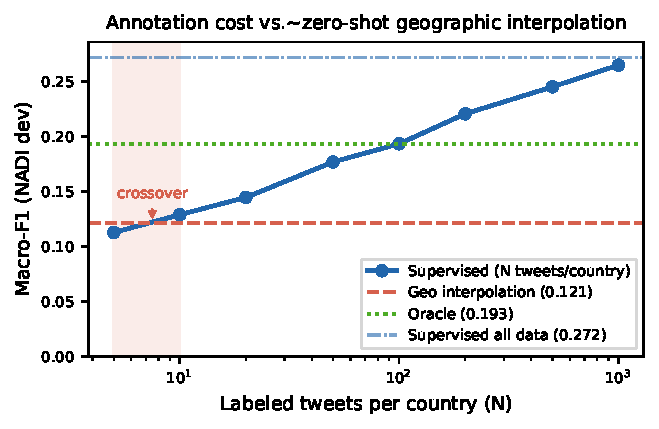
\includegraphics[width=\columnwidth]{figures/annotation_curve.pdf}
\caption{Supervised $n$-gram macro F1 vs.\ labeled tweets per Arabic variety (9 varieties with $\geq$1{,}000 training examples, means over 3 trials).
  Dashed: zero shot geo-interpolation baseline (0.121).
  Dotted: oracle full training (0.193).}
\label{fig:annot}
\end{figure}

Around 10 labeled tweets per variety beat the zero shot baseline on covered varieties.
Full oracle performance approaches at $N{=}1{,}000$.
Geographic interpolation matters most for varieties with no labeled data at all, the exact setting where annotation is most expensive or impossible.

%% ──────────────────────────────────────────────────────────────────────────────
\section{Analysis}
\label{sec:analysis}

\subsection{Does $r$ Predict Recovery? No.}
\label{sec:abs_r}

The natural hope is that $r$, which a practitioner can compute from unlabeled data alone, tells us in advance whether interpolation is worth deploying.
It does not.
Table~\ref{tab:abs_r} sorts the families by $|r|$.
The recovery column does not follow.

\begin{table}[t]
\centering
\small
\setlength{\tabcolsep}{5pt}
\begin{tabular}{lrrr}
\toprule
\textbf{Language} & $|r|$ & $r$ (sign) & \textbf{Recovery} \\
\midrule
Portuguese & 0.50 & $+$ & 33\% \\
Arabic     & 0.43 & $-$ & 63\% \\
Spanish    & 0.37 & $+$ & 26\% \\
Russian    & 0.33 & $+$ & 45\% \\
German     & 0.30 & $+$ & 57\% \\
French     & 0.14 & $-$ & 45\% \\
English    & 0.03 & $+$ & 48\% \\
\bottomrule
\end{tabular}
\caption{Absolute geographic--linguistic correlation $|r|$ and macro LOO recovery, sorted by $|r|$.
  Spearman($|r|$, recovery) $={-}0.21$, $p{=}0.65$.
  Spearman(signed $r$, recovery) $={-}0.71$, $p{=}0.07$.
  Neither gives a usable rule.}
\label{tab:abs_r}
\end{table}

\paragraph{Magnitude fails.}
The two families with the largest $|r|$, Portuguese (0.50) and Arabic (0.43), sit at opposite ends of the recovery range (33\% and 63\%).
English has almost no correlation ($|r|{=}0.03$) yet recovers 48\%, more than Russian, Spanish, and Portuguese, which all have much larger $|r|$.
The rank correlation between $|r|$ and recovery is $\rho{=}{-}0.21$ ($p{=}0.65$), indistinguishable from zero and, if anything, pointing the wrong way.
There is no $|r|$ threshold a practitioner could use.

\paragraph{Sign gives only a weak hint.}
The signed correlation does slightly better.
The two families with $r{<}0$, Arabic and French, both land in the upper half of the recovery range, which matches the original Tobler intuition that negative $r$ (nearby varieties more similar) is the helpful case.
But the trend is $\rho{=}{-}0.71$ at $p{=}0.07$, not significant at the 0.05 level with seven families, and German breaks it badly: $r{=}{+}0.30$ yet 57\% recovery, the second best.
The honest reading is that $r$ carries a faint directional signal and no usable magnitude signal.

\paragraph{Why the intuition fails.}
Recovery depends on how the held-out variety sits relative to its neighbors, which is a local property.
The correlation $r$ is a single global summary over all $\binom{V}{2}$ pairs.
A family can have a flat global $r$ yet still contain neighbor pairs that transfer well, as English and French show.
Conversely a high $|r|$ can come from a few distant pairs while the actual nearest neighbors transfer poorly, as in Portuguese, where Brazil dominates every mixture.
One number over the whole family cannot capture this.

\subsection{Register as a Confound}
\label{sec:register}

The Arabic and German contrast isolates the effect of \textbf{register}.
Both are in situ language families with centuries of change among neighboring varieties.
Yet Arabic shows negative geographic structure ($r{=}{-}0.43$) while German shows positive ($r{=}{+}0.30$).
The difference is the data source.

Twitter captures \emph{colloquial} Arabic.
Because of diglossia, speakers write in their own dialect rather than Modern Standard Arabic.
Peninsular Arabic, Levantine Arabic, and Maghrebi Arabic differ greatly in casual speech. mc4 captures \emph{formal written} German.
A speaker from Munich and a speaker from Zurich both produce Standard German when writing a blog post or news article.
Written standardization removes the regional signal that spoken registers keep.

This sign difference, though, does not translate into a recovery gap.
German recovers 57\% and Arabic 63\%, close despite opposite $r$.
Register shapes \emph{where} the geographic signal lives, but it does not let $r$ predict how well interpolation will do, which is the broader point of Section~\ref{sec:abs_r}.
The practical implication is narrow: colloquial data shows the Tobler pattern more cleanly, but formal data still supports a usable proxy.

%% ──────────────────────────────────────────────────────────────────────────────
\section{Discussion}
\label{sec:discussion}

\paragraph{Practical recommendation.}
For a new dialect variety with no labeled data, geographic interpolation is a reasonable first move.
It costs only unlabeled text and a table of centroids, and it recovers 26--63\% of oracle macro F1.
But do not expect $r$ to tell you in advance how well it will do.
We measured $r$ on the same unlabeled data and it did not predict recovery, in magnitude or in sign, strongly enough to act on.
Treat interpolation as a cheap baseline to try, not a method you can pre-screen.
The cheaper safeguard is a few labels.
On Arabic, around 10 labeled tweets per variety already beat the zero shot baseline (Section~\ref{sec:annotation}), so any variety that can be labeled at all is better served by a small seed set than by interpolation.

\paragraph{Beyond $n$-gram models.}
Geographic interpolation is not tied to a particular model type.
The same mixture approach (Eq.~\ref{eq:mixture}) can be applied to neural language models by interpolating output distributions or by averaging model parameters.
Applying it to fine tuned transformer models, such as CAMeLBERT \cite{inoue-etal-2021-interplay}, is a natural next step for Arabic.
Whether the same negative result about $r$ would hold for a neural mixture is an open question this paper does not answer.

\paragraph{Register and contact history.}
Two descriptive patterns help explain when the proxy works, even though neither rescues $r$ as a screening tool.
\emph{Register} shapes where the geographic signal lives: colloquial Twitter keeps the Tobler pattern (Arabic $r{<}0$) that Standard German web text flattens ($r{>}0$), though both still recover well (Section~\ref{sec:register}).
And \emph{contact history can override geography}: Lebanon recovers only 25\% despite a neighbor just 232\,km away (Section~\ref{sec:arabic}), a reminder that the mixture in Eq.~\ref{eq:mixture} encodes physical distance only, not the historical contact that actually shapes a dialect.

\paragraph{Future directions.}
Three extensions seem most direct.
The first is testing more language families and more varieties per family, since our central result is a non-correlation that a larger panel could in principle overturn.
The second is repeating the same protocol with neural models in place of character $n$-grams, interpolating output distributions or parameters instead of count-based probabilities, to see whether the same gap between local recovery and global correlation persists once the underlying model is more expressive.
The third is moving beyond country centroids toward finer-grained units, such as cities or provinces, which would let the method speak to the within-country variation we set aside in this study.
We see this work as a starting point for that agenda, not a closed result.

%% ──────────────────────────────────────────────────────────────────────────────
\section{Conclusion}
\label{sec:conclusion}

We tested geographic $n$-gram interpolation for zero shot dialect identification, first on Arabic and then across six more language families, covering 17 Arabic, 17 Spanish, 13 French, 11 English, 9 Russian, 5 German, and 3 Portuguese varieties.
The method works as a rough proxy everywhere, recovering 26--63\% of oracle macro F1 with no target labels, and does best on Arabic, at 63\%.

The main finding, though, is negative: the geographic--linguistic correlation $r$ does \emph{not} predict which families benefit.
Magnitude is useless (Spearman $|r|$ vs.\ recovery $\rho{=}{-}0.21$, $p{=}0.65$), and sign gives only a weak, non-significant hint that negative $r$ helps ($\rho{=}{-}0.71$, $p{=}0.07$).
A practitioner cannot screen families with $r$, even though it does help explain Arabic on its own.
The broader lesson is cautionary: geography gives a usable but unpredictable proxy for dialect transfer, and a single correlation is not enough to know in advance when it will pay off.
A single number, computed once on unlabeled data, is a tempting shortcut, but it is no substitute for measuring how a method actually performs on the variety at hand.

%% ──────────────────────────────────────────────────────────────────────────────
\bibliography{references}
\bibliographystyle{acl_natbib}

%% ──────────────────────────────────────────────────────────────────────────────
\section*{Limitations}

\paragraph{Arabic data quality.}
Arabic results rely on geotagged Twitter data, which has known biases.
Users declare their location manually, and many provide a city or country that does not reflect where they currently live.
Diaspora communities tweet in their heritage dialect from abroad, mixing a Moroccan dialect signal into a Belgian or French IP address.
Urban areas are overrepresented because Twitter usage is concentrated in cities, so rural and peripheral dialectal features are undersampled.
Code switching between Arabic and French, English, or local languages is common in Maghrebi and Peninsular tweets and adds noise to the $n$-gram profiles.

\paragraph{CC-TLD as a geographic proxy.}
The CC-TLD assumption maps a URL domain to a country of origin.
This is violated in several ways.
Multinational companies host content under a single national domain regardless of the intended audience.
Diaspora communities in Germany write in Arabic or Turkish under \texttt{.de} domains.
Bilingual countries like Belgium, Canada, and Switzerland produce mixed language content under a single CC-TLD.
International organizations and government sites often use national domains while writing in multiple languages.
Despite these violations, the aggregate signal across thousands of documents is consistent enough to produce useful $n$-gram profiles, but individual country profiles may be noisier than the numbers suggest.

\paragraph{Country centroids.}
We represent each country as a single geographic point.
This ignores within country dialect variation: Germany has northern and southern varieties, the United States has regional accents across thousands of kilometers, and Morocco spans Saharan and Atlantic coastal zones.
A more detailed geographic representation at the city or region level would likely improve results for large or geographically diverse countries.

\paragraph{Physical geography.}
Haversine distance measures straight-line distance between centroids on a sphere.
It ignores physical barriers that affect dialect diffusion: mountain ranges (Alps, Andes, Caucasus), bodies of water (Mediterranean, Atlantic), and political borders that restrict contact.
Lebanon and Palestine are 232\,km apart by Haversine distance but have had limited direct contact for decades.
A road distance or contact intensity measure might better predict linguistic similarity.

\paragraph{Small sample of families.}
Seven families is a small sample for a correlation claim.
Our central result is a non-correlation, so the risk runs the other way than usual: a real $r$ to recovery relationship could exist and stay hidden at $n{=}7$.
The signed-$r$ trend ($\rho{=}{-}0.71$, $p{=}0.07$) is suggestive but not significant, and German (5 varieties) and Portuguese (3 varieties) carry little weight on their own.
A larger panel of families, and more varieties per family, would test whether even the weak sign signal holds.

\paragraph{Protocol mismatch.}
Arabic is evaluated on an external benchmark (NADI 2020), while all other languages use intrinsic CC-TLD LOO.
These are not directly comparable.
The NADI benchmark uses informal social media text from a fixed test set with human-verified labels.
Intrinsic LOO uses the same noisy CC-TLD data for both training and testing.
Recovery numbers across languages should therefore be interpreted with care: a 63\% recovery for Arabic on a hard external benchmark is not the same experiment as a 57\% recovery for German on its own held-out web text.
This mismatch is also a reason not to over-read the cross-family correlation.

\paragraph{Model architecture.}
Character $n$-gram language models are simple and fast but miss word level and semantic variation.
Many dialectal differences are lexical, a word choice that marks a speaker as Jordanian or Kuwaiti, and $n$-gram models capture these only through partial character overlap.
Neural models trained on the same geographic data would likely achieve higher absolute performance and might show different $|r|$ behavior, particularly for families where lexical rather than phonological variation is the primary signal.

\paragraph{Coverage of world languages.}
We test seven language families, all using Latin, Arabic, or Cyrillic script.
The framework has not been tested on tone languages, agglutinative families, or languages with complex morphology such as Turkish, Swahili, or Mandarin Chinese.
The relationship between geographic proximity and linguistic similarity may be weaker or stronger in these families, and the register confound (colloquial vs.\ formal) may manifest differently.

\end{document}

